\documentclass[twocolumn]{article}

%\usepackage[francais]{babel}
\usepackage[T1]{fontenc}
\usepackage{amsmath}
\usepackage{color}
\usepackage{tikz}
\usepackage{subfig}
\usepackage[adobe-utopia]{mathdesign}

% Colors from famfamfam.com
\definecolor{vert}{HTML}{C1FF2D}
\definecolor{bleu}{HTML}{0BCEFF}
\definecolor{rose}{HTML}{FF0B5B}
\definecolor{gris}{gray}{0.7}

\usetikzlibrary{shapes,fit,calc}

\tikzset{line/.style={
    shorten >= -#1,
    shorten <= -#1}}
\tikzset{halfline/.style={
    shorten >= -#1}}
\tikzset{axe/.style={
    ->,
    thin}}
\tikzset{fig/.style={
    thick}}
\tikzset{origine/.style={
    draw=black,
    cross out}}
\tikzset{aabb/.style={
  dashed,
  thick,
  inner sep=0}}
\tikzset{gjknode/.style={
    fill=rose,
    circle}}
\tikzset{gjkedge/.style={
    draw=rose,
    thick}}
\tikzset{gjkdir/.style={
    halfline=0.5cm,
    draw=gris,
    very thick,
    dashed}}
\tikzset{gjkclosest/.style={
    circle,
    fill=bleu}}
\tikzset{rayon/.style={
    ->,
    draw=red}}

\newcommand{\deriv}{\partial \!}

\title{TITRE}
\author{Merwan Achibet}
\date{}

\begin{document}

\maketitle
\tableofcontents

\section{Introduction}

\subsection{Les moteurs physiques}

Invisibles, les phénomènes physiques qui régissent le fonctionnement
de notre univers sont pourtant omniprésents et universels. \'Etudiées
depuis des siècles, les lois les décrivant ont été à maintes reprises
redéfinies et affinées et il est de nos jours indispensable de pouvoir
les modéliser de façon fidèle ou tout du moins d'être capable de les
approximer de façon plausible.

Une simulation industrielle visant par exemple à reproduire
virtuellement les interactions entre les différentes pièces qui
composent une automobile doit être capable de reproduire de façon
réaliste la friction des pneumatiques sur le sol, l'influence de la
gravité sur le véhicule, le comportement thermique et volumique des
fluides qu'il contient ainsi que de nombreux autres aspects mécaniques
de son fonctionnement. Le système informatique simulant tous ces
facteurs est appelé moteur physique. Dans cet exemple, les enjeux de
sécurité et de qualité sont grands et des résultats d'une précision
extrême sont exigés. Les calculs à mettre en jeu pour les obtenir
peuvent donc se permettre d'être très coûteux et de se baser sur des
modélisations mathématiques complexes. Il n'est pas rare que ces
processus de simulation soient répartis sur plusieurs machines et
s'étalent sur une durée de calcul de plusieurs heures.

A contrario, les moteurs physiques d'autres types de système complexe
ne peuvent se permettre une telle latence et doivent fonctionner en
temps réel. La contrainte est encore plus forte lorsque le moteur
physique doit cohabiter avec d'autres modules gérant différents
aspects de l'application. On pense notamment aux jeux vidéo, qui
partagent le temps de calcul alloué entre le moteur graphique, le
moteur d'intelligence artificielle, la gestion du son, la gestion du
réseau, et bien sûr le moteur physique. Dans ce cadre, auquel on peut
greffer la réalité virtuelle et ses applications dérivées, la
contrainte la plus importante est le temps d'éxecution et non la
précision des résultats. On ne cherche plus à obtenir des données
exactes mais une représentation plausible du réel. Ainsi, certains
raccourcis pourront être tolérés et une part de réalisme est sacrifiée
au profit de la vitesse.

La physique est un champ très vaste dont les disciplines vont de
l'acoustique à l'électronique. Néanmoins, le spectre d'action des
moteurs physiques se limite à la mécanique classique, dite mécanique
newtonienne. Ce sous-domaine répond à des questions telles que :
Comment réagira cette balle si on la lance sur un mur ? Quelle est
l'influence d'une planète sur un objet spatial donné ? Pourquoi un
liquide visqueux dispose-t-il d'une faible vitesse d'écoulement ?
Quelles déformations engendrera un choc entre deux voitures ?

La mécanique newtonienne est elle-même une vaste discipline et la
précision d'une modélisation ne suffit pas à la différenciation entre
tous les moteurs physiques. Souvent, un moteur physique sera
spécialisé. Certains simuleront les interactions entre corps rigides
comme une boîte en plastique tombant sur le sol. Certains simuleront
le comportement d'objets déformables comme deux véhicules se
percutant. D'autres se concentreront sur les réactions entre liquides
ou entre gaz.

\subsection{Travail à accomplir}

L'objectif de ce projet est de concevoir un moteur physique de base
permettant de gérer les interactions entre des corps rigides et
convexes. On parle de corps rigides dans la mesure o\`u les objets mis
en jeu seront indéformables et incassables. Dans un tel contexte, une
tasse en porcelaine surmontée d'un bloc de granite d'une tonne ne
serait aucunement endommagée. On parle de corps convexes car se
limiter dans un premier temps à ce type de structure autorise
certaines facilités dans les calculs. Une piste pour étendre la
simulation aux solides concaves est de décomposer un corps concave en
plusieurs corps convexes.

La contrainte principale de notre application sera le temps. On veut
concevoir une simulation éxecutable en temps réel de telle façon que
si l'utilisateur modifie l'environnement de la simulation à un instant
quelconque, une réaction à cette interaction soit immédiatement
perceptible. Bien que certains raccourcis dans les calculs ainsi que
plusieurs approximations soient acceptés, le fonctionnement du moteur
se base sur des lois bien connues de la mécanique de Newton et ses
résultats ne devront pas s'éloigner de façon demesurée de ceux que
l'on retrouverait dans une situation réelle.

\subsection{\'Etude de cas}

L'activité physique d'un corps se divise en plusieurs phases. Afin de
les détailler, analysons une situation concrète. Si l'on tenait une
balle dans notre main et que nous la lâchions au dessus d'un plan,
quelles seraient les étapes que cet objet traverserait avant d'arriver
à un état de repos ?

\subsubsection{La chute}

La main s'ouvre et laisse s'échapper la balle. Notre appréhension du
monde qui nous entoure nous permet de prévoir intuitivement que
l'objet tombera et accélérera vers le bas. Ce phénomène est quantifié
par la seconde loi de Newton.
\begin{align*}
  \vec{a} = \frac{1}{m} \sum_i \vec{F}_i
\end{align*}

Cette règle décrit l'accélération $\vec{a}$ d'un corps comme étant le
produit de l'inverse de sa masse $m$ et de la somme des forces
$\vec{F}_i$ qui lui sont appliquées. Dans notre exemple, on lâche la
balle sans lui donner d'élan initial et la seule influence qu'elle
subit au cours de sa chute est celle de la gravité. La gravité
terrestre est une force de $9.81 \times m$ newtons (avec $m$ la masse de la
balle) dirigée vers le noyau de la planète mais dans la simulation, on
peut la réduire à une force dirigée vers le bas (dans la direction
négative de l'axe $y$). Afin de bénéficier d'un moteur physique
versatile, la puissance de la gravité pourra être modifiée, pour
simuler une situation lunaire par exemple, ou être totalement annulée,
pour simuler une situation d'apesanteur. En réalité, la gravité ne
sera même pas codée \og en dur \fg{} mais appartiendra à une liste de
forces environnementales qui contiendra toutes les influences que le
monde de la simulation fait subir aux corps qu'il contient. On pourra
par exemple modéliser la résistance de l'air ou la poussée irrégulière
du vent.

Cette observation du comportement de la balle nous oriente sur la
façon dont l'on pourra modéliser les déplacements d'objets soumis à
des forces extérieures. \`A chaque corps seront associées des
quantités physiques telles que la position, la vitesse et
l'accélération. Le rôle principal du moteur physique sera de faire
évoluer ces variables de façon à ce que le résultat d'une simulation
s'approche le plus possible de ce qui serait observable dans le monde
réel. Dans la première partie de ce compte-rendu, on précisera donc
les méthodes employées pour simuler la dynamique des corps.

\subsubsection{Le rebond}

Alors que la balle s'approche du plan, on s'attend naturellement à ce
qu'elle entre en contact avec ce dernier et qu'une réaction
proportionnelle à la puissance du choc soit produite. Cette réaction
dépend de nombreux facteurs, notamment des masses des objets
considérés et de leur vitesse respective.

Le moteur physique devra être capable de générer une réaction réaliste
dont la détermination passe par une formule présentée dans la seconde
partie. Néanmoins, le travail le plus complexe n'est pas de calculer
une réponse mais de détecter une collision. Plusieurs processus
géométriques devront être mis en place afin de vérifier si une
collision a lieu et si tel est le cas, afin de mesurer précisément
quels points des deux corps entrent en contact.

Une difficulté supplémentaire vient du fait que la simulation est mise
à jour de façon discrète, par pas de temps fixe. Lorsqu'une collision
sera détectée entre deux corps, il est presque impossible de se
retrouver dans une situation de contact parfait. On aura plutôt des
contacts pénétrants au sein desquels l'intégrité physique des corps
est corrompue et les objets rentrent l'un dans l'autre. Une des tâches
du moteur physique sera de pallier ce problème en recalant les corps
dans la position de contact parfait qu'ils auraient dû atteindre.

Cette phase de la vie d'un corps rigide est la plus courte,
puisqu'instantanée, mais demandera paradoxalement le plus de
travail. Les considérations géométriques qui entrent en jeu, ainsi que
les limites à contourner, imposées par l'arithmétique des nombres à
virgule flottante, seront détaillées dans la seconde section.

\subsubsection{Le repos}

Les rebonds sur le plan sont de plus en plus faibles, jusqu'à ce que
la balle n'ait plus assez d'énergie cinétique pour s'élever à
nouveau.

Son état de repos laisse penser que plus aucune force ne s'applique
sur elle. Contrairement aux apparences, dans le monde réel ce n'est
pas parce qu'un corps est fixe qu'il est libre de toute influence. La
gravité n'a pas disparu par magie et pourtant l'accélération de la
balle est nulle, puisqu'elle reste immobile. La troisième loi de
Newton \cite{newton} est là pour démystifier cette situation :

\begin{quote}
\textit{Tout corps $A$ exerçant une force sur un corps $B$ subit une force
d'intensité égale, de même direction mais de sens opposé, exercée par
le corps $B$.}
\end{quote}

Autrement dit :
\begin{align*}
  &\vec{F}_{A/B} = -\vec{F}_{B/A} \\
  &\vec{F}_{A/B} + \vec{F}_{B/A} = 0
\end{align*}

Ici, la balle subit toujours la gravité mais le plan produit une force
inverse qui permet d'annuler tout mouvement. Même si un spectateur
aura l'impression que la balle est inactive, son état collisionel
constant lui permet de rester à la surface du plan et d'équilibrer le
système. Ce phénomène sera reproductible dans le moteur physique et
sera basé sur la même méthode que les collisions classiques.

Puisque l'une des préoccupations majeures de ce projet est la vitesse
d'exécution, d'autres considérations plus techniques entreront elles
aussi en jeu. Une fois qu'un objet est immobile, par exemple, peut-on
le fixer artificiellement et ne plus faire évoluer son état pour
économiser des ressources ? Si tel est le cas, quand devra-t-on à
nouveau le rendre mobile ?

\section{Dynamique} 

\subsection{La composante linéaire du mouvement}

Nous allons pour l'instant nous concentrer sur l'aspect cinématique d'un corps rigide, c'est à dire son mouvement lorsqu'il n'est soumis à aucune force extérieure. Dans un premier temps, seule la composante linéaire du mouvement sera étudiée et les objets dont nous allons simuler le comportement seront réduits à de simples particules. Les figures présentées sont en deux dimensions pour des raisons de clarté mais le principe reste similaire lorsqu'il est étendu à la troisième dimension.

La quantité physique la plus perceptible visuellement pour un spectateur est la position $p$ d'un corps. Pour notre affichage final, c'est cette valeur à tout instant $t$ de la simulation que l'on veut déterminer. Le travail de cette partie du moteur physique revient donc à déterminer la nouvelle position d'un objet à partir de la connaissance des forces qui lui sont appliquées. Un corps possède aussi une vitesse $v$, qui correspond à la variation de sa position pour une unité de temps. On note cette relation sous la forme dérivée :

\[\vec{v} = \frac{\delta \vec{p}}{\delta t}\]

Pareillement, l'accéleration $a$, qui apparaissaît plus tôt dans la seconde loi de Newton, correspond à la variation de la vitesse par rapport à une unité de temps.

\[\vec{a} = \frac{\delta \vec{v}}{\delta t}\]

Par transitivité, on confirme que la position est dépendante de l'accélération.

\[\vec{a} = \frac{\delta \vec{v}}{\delta t} = \frac{\delta^2 \vec{p}}{\delta t}\]

Grâce à cette équation, on peut calculer l'accélération d'un objet à partir de sa variation de position. Dans le moteur physique, ce sera en fait l'opération inverse qui devra être effectuée : on connaîtra les forces appliquées, on en déduira l'accélération induite par la seconde loi de Newton puis on calculera le changement de position. Il faut donc exploiter le fait que ces trois quantités partagent aussi des relations de primitive.

\[\vec{p} = \int \vec{v}\; \delta t = \int \vec{a}\; \delta t^2\]

Récapitulons. Chacun des corps rigides dont l'on veut simuler l'évolution possèdera ces trois quantités sous forme vectorielle et l'une des tâches de base du moteur physique sera de traduire l'application de forces en un changement de position. On sait qu'elles entretiennent des relations de dérivation, il faudra donc procéder par intégration pour calculer la position d'un objet à partir de son accélération.

\subsection{Intégration}

Dans la sous-section précédente, les trois quantités physiques entrant en jeu dans les mouvements linéaires ont été présentées. \'Etudions maintenant de façon plus concrète sur quels calculs se basera la partie la plus élémentaire du moteur physique.

Les phénomènes mécaniques du monde réel évoluent de façon continue mais notre simulation ne peut pas s'autoriser ce luxe. Le modèle du moteur physique sera donc discret et avancera par pas de temps fixe $\delta t$. \`A chaque mise à jour de la simulation, des intégrations doivent être réalisées pour déterminer le changement d'état d'un corps d'un instant $t_n$ à un instant $t_{n+1}$. Toujours pour des raisons d'efficacité, nous ne pouvont pas nous permettre d'allouer un temps de calcul trop important à cette phase de la mise à jour et nous devons trouver un moyen d'approximer ces intégrales.

Parmi les techniques classiques d'intégration approximative, on trouve l'intégration d'Euler. Cette méthode part du principe que l'on dispose de la valeur initiale $x_0$ de la quantité que l'on souhaite faire évoluer ainsi que de son taux de changement $x'$ et de la variation de temps par rapport à l'état précédent.

\[x_{n+1} = x_{n} + x' \delta t\]

Si l'on adapte cette idée à notre problème, on obtient la succession de calculs suivante :

\[a_{n+1} = \frac{\sum \vec{F}_i}{m}\]
\[\vec{v}_{n+1} = \vec{a}_n + \vec{a}_{n+1} \delta t\]
\[\vec{p}_{n+1} = \vec{p}_n + \vec{v}_{n+1} \delta t\]

On calcule l'accélération à un instant $t$ puis on intègre en fonction du temps jusqu'à obtenir la nouvelle position du corps. Ce processus doit être repété à chaque mise à jour du système et ce, pour chaque corps. On aurait pu choisir une autre méthode d'intégration, telle que l'intégration Runge-Kutta d'ordre 4 qui divise un pas de temps en plusieurs segments, ou bien telle que l'intégration de Verlet qui dispose d'une meilleure stabilité, mais Euler reste le choix le plus économique et fournit des résultats relativement corrects.

Afin de réduire la complexité de la structure informatique qui représentera un corps rigide, nous allons introduire la notion d'élan linéaire. Pour un corps rigide, l'élan linéaire $\vec{L}$ est le produit de la masse et de la vitesse. Cette nouvelle quantité a pour avantage majeur de posséder comme primitive la variation de force exercée sur le corps.

\[{\sum \vec{F}_i} = \frac{\delta \vec{L}}{\delta t} = \frac{\delta (m\vec{v})}{\delta t}\]

Ce qui signifie que l'on peut réduire l'intégration de l'état d'un corps à :

\[\vec{L}_{n+1} = \vec{L}_n + {\sum F}\]
\[\vec{p}_{n+1} = \vec{p}_n + \frac{\vec{L}_{n+1}}{m} t\]

L'élan linéaire remplace l'accélération dans la définition d'un corps et permet de calculer sa vitesse. Cette organisation permet à première vue une intégration plus courte mais les avantages majeurs de ce choix prendront tous leurs sens lorsque le mouvement angulaire sera introduit.

\subsection{Modélisation d'un corps rigide}

Nous avons décrit dans la partie précédente les quantités régissant le mouvement linéaire d'une particule ainsi que la façon dont elles évoluent mais le moteur physique que l'on conçoit a pour visée de simuler les interactions entre des corps rigides à volume convexe. Comment peut-on étendre les principes énoncés pour des particules à ce modèle ?

On pourrait en premier lieu penser à représenter un tel corps par une liste de particules, chacune placée à un coin de l'objet. Chaque particule évoluerait indépendement et des contraintes de cohésion entre particules voisines seraient appliquées pour empêcher toute déformation du corps. Cette méthode est envisageable mais elle présente plusieurs désavantages. Premièrement, les règles de cohésion à mettre en place nécessiteraient des traitements supplémentaires, et donc un temps de calcul plus élevé. Deuxièment, un corps devrait passer par autant d'intégrations qu'il a de points à chaque mise à jour. Il existe une solution plus simple et plus élégante qui permet de réduire les mouvements linéaires d'un corps rigide à ceux d'une unique particule judicieusement placée.

Introduisons en premier lieu la notion de repères absolu et local. Le repère absolu est le référentiel orthogonal dont l'origine sert de centre à l'environnement de la simulation. Un repère local est un référentiel qui est unique à chaque corps et dont le centre se situe à l'intérieur même de cet objet.

\begin{tikzpicture}
  % repère
\draw[axe] (-0.2,0) -- (10,0);
\draw[axe] (0,-0.2) -- (0,10);


  % figure
  \coordinate (C) at ++(6,5);
  \draw (C) circle (2);

  % repère local  
  \begin{scope}[rotate around={-30:(C)}]
    \draw[->] (C) -- +(4,0);
    \draw[->] (C) -- +(0,4);
  \end{scope}
\end{tikzpicture}


La position exacte du repère local dépend de la position des points qui forment l'objet mais il ne s'agit pas d'un simple centre géométrique puisque la masse de chaque point est aussi un facteur déterminant. Cette position se nomme le centre de masse, ou barycentre, et sera calculée par la formule suivante, o\`u $M$ représente la masse totale des points, et $m_i$ et $\vec{p}_i$ respectivement la masse et la position dans le repère absolu du point $i$.

\[C = \frac{1}{M} \sum m_i \vec{p}_i\]

Une fois le centre de masse défini, la position locale $\vec{r}_i$ d'une particule $i$ peut être calculée en fonction de sa position absolue $\vec{p}_i$ par :

\[\vec{r}_i = \vec{p}_i - C\]

Le processus de définition d'un corps se déroule comme suit :
\begin{enumerate}
  \item{L'utilisateur entre les points de l'objet un par un, dans le repère absolu}
  \item{L'utilisateur renseigne les points qui sont reliés par des arête afin de former les faces de l'objet}
  \item{Le centre de masse est automatiquement calculé avant la simulation}
\end{enumerate}

Grâce au centre de masse, on a une seule position à faire évoluer, quelle que soit la compléxité de la structure du corps concerné.

\subsection{La composante angulaire du mouvement}

Le modèle que nous avons défini est encore incomplet puisqu'il ne prend pas en compte la composante rotationnelle des mouvements dont l'on peut être témoin dans un environnement réel. Les particules étant de simples points flottants dans l'espace, cela ne posait pas de problème précédemment mais le moteur physique que l'on conçoit doit gérer des corps rigiques plus complexes. Imaginons une boîte cubique que l'on lancerait en l'air, si aucune rotation n'apparaît (si la base de la boîte reste parallèle au sol), l'imitation du réel que l'on souhaite reproduire perd toute crédibilité.

Les quantités physiques entrant en jeu dans la décomposition d'un déplacement angulaire sont analogues à celle présentées dans la partie traitant de la dynamique linéaire : à la position et à l'élan linéaire correspondent l'orientation et l'élan angulaire.

\subsubsection{L'orientation}

De la même façon que la position représentait visuellement l'état d'un corps au sein de la composante linéaire, un corps doit posséder une orientation. En deux dimensions, un nombre flottant représentant l'angle du corps par rapport à un axe fixe suffirait à décrire l'orientation d'un objet mais pas dans notre environnement en trois dimensions.

Le repère local d'un corps a été introduit dans la partie précédente et se résumait à un centre de masse faisant office d'origine, mais un repère possède aussi des axes et ceux du repère local ne sont pas nécessairement alignés avec ceux du repère absolu. Pour représenter la direction des axes du repère local, et donc l'orientation, on utilisera une matrice de dimension trois au sein de laquelle chaque vecteur colonne correspondra à un des axes du repère local \cite{witkit97}. Pour illustrer ces propos, analysons la matrice d'orientation égale à la matrice d'identité d'ordre 3.

\[
\begin{pmatrix}
  1 & 0 & 0 \\
  0 & 1 & 0 \\
  0 & 0 & 1
\end{pmatrix}
\rightarrow
\begin{pmatrix}
  1 \\
  0 \\
  0 
\end{pmatrix}
\begin{pmatrix}
  0 \\
  1 \\
  0 
\end{pmatrix}
\begin{pmatrix}
  0 \\
  0 \\
  1 
\end{pmatrix}
\]

Si l'on isole les vecteurs colonnes de cette matrice identité, on remarque que chacun correspond à un des axes du repère global. Le premier vecteur colonne d'une matrice d'orientation correspond donc à l'axe $x$ du repère local. Il en est de même pour la seconde colonne avec l'axe $y$ et la troisième colonne avec l'axe $z$.

\subsubsection{\'Elan angulaire}

Il nous faut désormais représenter le taux de variation de l'orientation d'un corps. La vitesse angulaire sera représentée par un vecteur dont la direction correspondra à l'axe autour duquel le corps effectuera sa rotation et dont la magnitude représentera le nombre de rotations à effectuer en une unité de temps. La relation entre orientation et élan angulaire est plus complexe que celle reliant position et élan linéaire.

intégration

torseur inertie

skew

reorthogonalisation

etc

\section{Gestion des collisions}

\subsection{Le cas des sphères}

\subsubsection{Détection du point de contact}

Nous allons dans un premier temps réduire le problème collisionnel aux interactions entre sphères. On sait que deux corps sont en collision si la distance qui sépare leurs centres est inférieure à la somme de leurs rayons. Cette simplification nous permet de nous concentrer sur la détermination des points de contact réels et d'éluder de nombreuses complications géométriques.

\`A chaque itération de la simulation, les corps présents dans l'environnement du moteur physique sont susceptibles de se déplacer et donc d'entrer en contact. Le moteur simule ces évolutions de manière non continue et il est très improbable qu'une collision soit détectée au moment précis o\`u elle se produit. On est donc régulièrement témoin de situations d'inter-pénétration au sein desquelles des corps rentrent l'un dans l'autre.

DESSIN t0 sphères éloignées, t1 sphères interpénétrées

On pourrait se satisfaire de cette imprécision et calculer les forces de rebond appropriées mais plusieurs situations critiques risquent d'apparaître. La force de séparation génération ne pourrait pas être suffisante pour séparer entièrement les deux sphères, ce qui les bloqueraient balbla. Pour trouver le point de contact réel entre deux sphères, il existe plusieurs approches. Les systèmes qui préfèrent favoriser le temps d'éxécution au détriment du réalisme se contente de repositionner les corps à un point de contact calculé par interpolation en fonction du temps de la dernière ntégration. Il est évident que des objets sujets à des déplacements non linéaires (variation de la vitesse pendant un pas de temps, trajectoire elliptique) seront mal replacés.

Même si la vitesse d'éxecution est un facteur important dans nos choix de conception, nous allons prendre un chemin différent et sélectionner une méthode plus précise qui fonctionnera par retour en arrière. La fonction d'intégration du moteur prend comme seul argument le pas de temps duquel faire avancer la simulation et pour l'instant on utilisait un pas constant. Or, une caractéristique intéressante de cette fonction et qu'elle peut prendre en argument un pas de temps négatif et simuler en sens inverse ! Grâce à cette caractéristique, dés qu'une inter-pénétration est détectée, on peut revenir en arrière jusqu'à retrouver le temps de contact exact. Le terme "exact" est à prendre avec des pincettes puisque notre simulation est limité par l'arithmétique des nombres à virgules flottantes et que l'on devra se contente d'un résultat quasi-exact, validé par un seuil de tolérance adapté.

Afin d'accélérer cette phase de recherche de la configuration de contact, le retour en arrière se fera par dichotomie. On recule en premier lieu de la moitié du pas de temps puis, si l'inter-pénétration est toujours présente, on recule d'un quart du pas de temps, sinon on avance d'un quart du pas de temps, et ainsi de suite jusqu'à obtenir une précision satisfaisante.

DESSIN

Une fois ce processus achevé, la configuration de contact est retrouvé et les deux sphères ne sont plus en situation de pénétration mutuelle. Il reste à déterminer quelles forces appliquer aux corps pour qu'ils se séparent.

\subsubsection{Réponse à une collision}



\subsection{Le cas général des corps rigides}

\subsubsection{Détection précise d'une collision}

Nous avons vu comment détecter une collision entre deux sphères, retrouver la configuration au temps de contact et les faire réagir de façon réaliste. Le procédé à suivre pour appliquer le même traitement à des corps rigides généralisés se base sur les mêmes principes mais nécessite des méthodes différentes, notamment du fait de leur structure géométrique plus complexe.

Si pour les sphère on détectait une collision en comparant la distance entre les centres et la somme des rayons, il faudra utiliser une autre technique pour les polyhèdres. Heureusement, une loi géométrique naturelle va permettre de vérifier ce prédicat de manière simple et rapide. Cette loi dicte que deux corps ne sont pas en situation d'interpénétration s'il existe dans l'espace un plan les séparant. On nommera un tel plan, plan de séparation.

En cas de non collision, il existe une infinité de plan de séparation entre deux polyhèdres mais on peut se limiter à vérifier les plans prolongeant les faces de chaque corps.

DESSIN

L'algorithme de détection d'une collision suivra donc le mode opératoire suivant :

interpenetration(p1, p2)
-pour toutes les faces de p1
--pour tous les vertex de p2
---si v du mauvais côté
----retourne vrai
-retourne faux

r=i(p1, p2) || i(p2, p1)

Cette méthode a pour avantage de savoir de manière certaine si deux polyhèdres sont entrés en collisions ou non mais sa complexité est de mauvaise augure pour la vitesse générale du moteur physique. Des corps composés de peu de faces, des boîtes par exemple, ne poseront pas de problème, mais des polyhèdres plus complexes risquent de ralentir fortement la détection d'une collision (une nouvelle raison d'avoir traîté le problème des sphères de façon différente). Si l'on ajoute à ce problème le fait que cette procédure est subit par chaque corps à chaque itération, blabla.

\subsubsection{Détection d'une collision potentielle}

Une méthode déterminant de façon certaine si des corps sont en contact a été présentée mais malgré la certitude de ses résultats, elle est trop coûteuse pour être utilisée pour chaque corps et à chaque itération. Nous allons utiliser une seconde technique de détection qui nous renseignera sur la possibilité d'une collision. Elle sera moins précise mais beaucoup plus économique. C'est seulement quand cette méthode nous avertira d'une collision possible que l'on utilisera la méthode plus coûteuse des plans de séparation.

La méthode se basera sur l'utilisation de boîtes englobantes, ou \textit{bounding boxes}. Chaque corps est associé à une boîte que le contient entièrement et est alignée par rapport aux axes du repère global (on parle d'\textit{AABB}, pour \textit{axis-aligned bounding-box}). 

\subsubsection{Détection du point de contact}

\subsubsection{Réponse à une collision}

\section{Le moteur physique}

\subsection{Algorithme général}

Nous disposons désormais des briques de base nécessaires à la
construction de l'algorithme général du moteur physique. Un appel à
cette procédure intégrera les états de tous les corps de la simulation
d'un pas de temps $\deriv t$ en tenant compte des interactions
possibles. On part de l'hypothèse que tous les corps sont initialement
séparés et donc qu'aucune interpénétration ne se produit au départ.

En premier lieu, on vérifie pour chaque paire de corps s'ils entrent
en collision. Si tel est le cas, on corrige leur état puis on applique
les impulsions adaptées. Ensuite, on administre des forces
environnementales, telles que la gravité. Il ne reste plus qu'à
intégrer l'état de tous les corps, c'est à dire mettre à jour leurs
position et orientation en fonction des élans transmis par les
impulsions et les forces extérieures. L'algorithme \ref{algoMoteur1}
résume cette organisation.

\begin{algorithm}[h]
  \caption{Boucle principale}
  \label{algoMoteur1}
  \dontprintsemicolon
  \SetKwData{pairedecorps}{paire de corps}
  \SetKwData{contact}{contact}
  \SetKwData{corps}{corps}
  \SetKwFunction{collisionGrossiere}{collisionGrossiere}
  \SetKwFunction{collisionFine}{collisionFine}
  \SetKwFunction{corrigerCollision}{corrigerCollision}
  \SetKwFunction{detecterContacts}{detecterContacts}
  \SetKwFunction{calculerImpulsion}{calculerImpulsion}
  \SetKwFunction{appliquer}{appliquer}
  \SetKwFunction{appliquerForcesEnvironnementales}{appliquerForcesEnvironnementales}
  \SetKwFunction{integrer}{integrer}
  \Entree{Un pas de temps $\deriv t$}
  \BlankLine
  \PourCh{\pairedecorps (A,B)}{
    \Si{\collisionGrossiere{A,B}}{
      \Si{\collisionFine{A,B}}{
        \corrigerCollision{A,B}\;
        $C \leftarrow$ \detecterContacts{A,B}\;
        \PourCh{\contact $c \in C$}{
          $I \leftarrow$ \calculerImpulsion{c}\;
          \appliquer{I, A}\;
          \appliquer{-I, B}\;
        }
      }
    }
  }
  \BlankLine
  \PourCh{\corps A}{
    \appliquerForcesEnvironnementales{A}\;
    \integrer{A, $\deriv t$}
  }
  \BlankLine
\end{algorithm}

Cette structure simple fonctionne de façon satisfaisante lorsque la
simulation comporte peu d'objets. Néanmoins, sa stabilité est
fortement compromise lorsque de nombreux corps entrent en jeu et ce,
pour plusieurs raisons.

Depuis le début de la conception du moteur physique, nous détectons,
corrigeons et traîtons les collisions entre paire de corps. On part de
l'hypothèse qu'au début de la simulation aucun solide n'entre en
collision avec un autre et grâce à la phase de correction
collisionnelle, cette hypothèse est vérifiée au début de chaque
intégration. Un problème majeur de l'algorithme actuel est qu'il
provoque des situation d'interpénétration non corrigeables, notamment
lorsque des amas d'objets se forment. La sous-figure $a$ de la figure
\ref{probleme} prend place au début d'une itération de la simulation.
On y voit un corps $A$, attiré par la gravité, et s'étant enfoncé dans
le sol. Le corps $B$ subit quand à lui la même influence mais ne tombe
pas assez bas pour qu'une collision avec $A$ s'opère. La sous-figure
$b$ nous montre le résultat de la correction de l'interpénétration
entre $A$ et le sol et on remarque qu'une nouvelle collision entre $B$
et $A$ en découle. L'issue de cette situation dépend de $B$; si sa
phase de détection de collision est déjà passée alors il est déjà trop
tard et $A$ et $B$ seront en état d'interpénétration à l'itération
suivante et l'hypothèse de non-pénétration ne sera pas respectée. Le
comportement de la simulation sera alors imprévisible. La stabilité du
moteur physique est donc gravement dépendante de l'ordre arbitraire
dans lequel les corps sont rangés et exécutent leur détection de
collision.

\begin{figure}
  \centering
  \subfloat[]{ 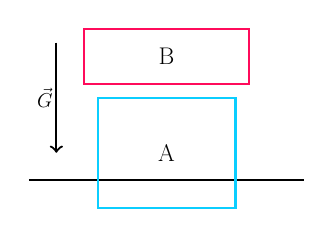
\begin{tikzpicture}[scale=0.35,transform shape]
  \draw[black,thick] (0,0) -- (10,0);

  \draw[->,thick,black,font=\huge] (1,5) to node[black,auto,swap] {$\vec{G}$} (1,1);

  \node[
    rectangle,
    minimum width=5cm,
    minimum height=4cm,
    draw=bleu,
    thick] at (5,1) (a) {};

  \node[font=\Huge] at (a.center) (al) {A};

  \node[
    rectangle,
    minimum width=6cm,
    minimum height=2cm,
    draw=rose,
    thick] at (5,4.5) (b) {};

  \node[font=\Huge] at (b.center) (bl) {B};

\end{tikzpicture}
 }
  \subfloat[]{ 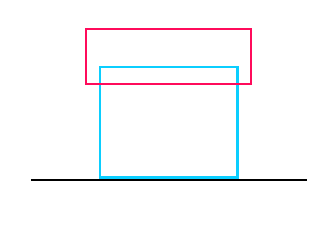
\begin{tikzpicture}[scale=0.35,transform shape]
  \draw[black,thick] (0,0) -- (10,0);


  \node[
    rectangle,
    minimum width=5cm,
    minimum height=4cm,
    draw=bleu,
    thick] at (5,2.1) (a) {};

  \node[
    rectangle,
    minimum width=6cm,
    minimum height=2cm,
    draw=rose,
    thick] at (5,4.5) (b) {};

  \node[
    rectangle,
    minimum height=1cm] at (0,-0.53) (s) {};

\end{tikzpicture}
 }
  \caption{Interpénétration collatéralement provoquée par une correction collisionnelle}
  \label{probleme}
\end{figure}

De plus, l'organisation actuelle prive la simulation de toute
cohérence temporelle. En effet, à chaque itération tous les corps
avancent d'un pas de temps fixe $\deriv t$ mais l'état de ceux
subissant une collision sera inmanquablement corrigé pour correspondre
à l'état qu'ils auraient dû atteindre au moment du contact. On se
retrouve ainsi avec des corps n'ayant pas subi de collision, côtoyant
des corps en ayant subit et dont l'état correspond à un temps
précédent.

Autre problème de taille : la simulation empruntera des chemins
différents selon l'ordre dans lequel les collisions sont détectées. La
figure \ref{issues} nous montre deux corp ainsi que la position qu'ils
atteindraient à l'itération suivante si l'on ignorait les collisions
(en pointillés). On peut aisément se rendre compte des conséquences de
l'ordre dans lequel les objets sont traîtés. Si le corps bleu est
traîté en premier, il entrera en collision avec le corps rose, son
état sera corrigé, et une impulsion sera plus tard générée pour
séparer les deux corps. Au final, l'objet bleu sera projeté vers la
gauche et le corps rose sera dévié de sa trajectoire originelle. Par
contre, si c'est le corps rose qui est traîté en premier, il avancera
vers sa prochaine position, puis ce sera autour de l'autre corps de se
déplacer. Puisque le corps rose ne se trouvera plus sur sa
trajectoire, rien ne se passera !

\begin{figure}
  \centering
  \subfloat{ 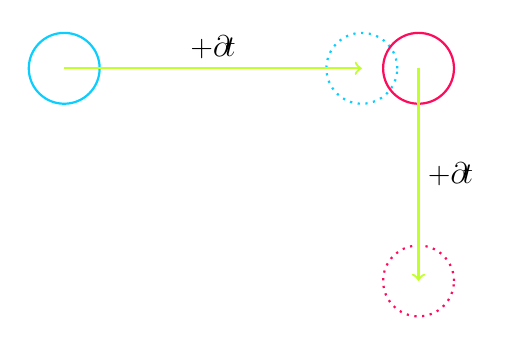
\begin{tikzpicture}[scale=0.9,transform shape]
  \coordinate (A1) at (0,0);
  \coordinate (A2) at (4.2,0);
  \coordinate (B1) at (5,0);
  \coordinate (B2) at (5,-3);

  \node[
    circle,
    minimum size=1cm,
    draw=bleu,
    thick] at (A1) (a1) {};
  \node[
    circle,
    minimum size=1cm,
    draw=bleu,
    thick,
    dotted] at (A2) (a2) {};
  \draw[->,thick,vert,font=\large] (A1) to node[black,auto] {$+ \deriv t$} (A2);

  \node[
    circle,
    minimum size=1cm,
    draw=rose,
    thick] at (B1) (b1) {};
  \node[
    circle,
    minimum size=1cm,
    draw=rose,
    thick,
    dotted] at (B2) (b2) {};
  \draw[->,thick,vert,font=\large] (B1) to node[black,auto] {$+ \deriv t$} (B2);

\end{tikzpicture}
 }
  \caption{Deux issues possibles selon l'ordre du traitement des collisions}
  \label{issues}
\end{figure}

Tous les problèmes cités sont clairement liés à un manque de cohérence
temporelle. Lors de l'utilisation d'un tel algorithme, on utilise un
pas de temps dit explicite \cite{garstenauer}. Nous allons maintenant
nous tourner vers une version améliorée, dont le pas de temps sera dit
implicite.

L'algorithme \ref{algoMoteur2} est plus solide dans la mesure o\`u il
détecte à chaque itération le temps du premier contact et intègre tous
les corps de la simulation jusqu'à cet instant de façon à traîter les
collisions dans leur ordre réel. Détaillons le fonctionnement de cette
nouvelle méthodologie. En premier lieu, on copie chaque corps afin de
s'assurer que les modifications qui vont suivre ne changent pas leur
véritable état de départ. On avance ensuite l'état de chaque copie
pour détecter si une collion se produira avec l'autre. Si tel est le
cas, on corrige la pénétration et on détermine les informations de
contact. \`A la fin de cette phase de prédiction, on dispose d'une
liste de contacts potentiels qu'il est nécessaire de trier en fonction
du temps d'impact. On intègre l'état de tous les objets d'un pas de
temps égal au plus faible temps d'impact.

\begin{algorithm}[h]
  \caption{Boucle principale améliorée}
  \label{algoMoteur2}
  \dontprintsemicolon
  \SetKwData{pairedecorps}{paire de corps}
  \SetKwData{contact}{contact}
  \SetKwData{corps}{corps}
  \SetKwFunction{collisionGrossiere}{collisionGrossiere}
  \SetKwFunction{collisionFine}{collisionFine}
  \SetKwFunction{corrigerCollision}{corrigerCollision}
  \SetKwFunction{detecterContacts}{detecterContacts}
  \SetKwFunction{calculerImpulsion}{calculerImpulsion}
  \SetKwFunction{appliquer}{appliquer}
  \SetKwFunction{integrer}{integrer}
  \SetKwFunction{trierContacts}{trierContacts}
  \SetKwFunction{appliquerForcesEnvironnementales}{appliquerForcesEnvironnementales}
  \SetKwFunction{mint}{min}
  \Entree{Un pas de temps $\deriv t$}
  \BlankLine
  $C \leftarrow \emptyset$\;
  \PourCh{\pairedecorps (A,B)}{
    $A_2 \leftarrow A$\;
    $B_2 \leftarrow B$\:
    \appliquerForcesEnvironnementales{$A_2$}\;
    \integrer{$A_2$, $\deriv t$}
    \appliquerForcesEnvironnementales{$B_2$}\;
    \integrer{$B_2$, $\deriv t$}
    \BlankLine
    \Si{\collisionGrossiere{$A_2$, $B_2$}}{
      \Si{\collisionFine{$A_2$, $B_2$}}{
        \corrigerCollision{$A_2$, $B_2$}\;
        $C \leftarrow C \cup$ \detecterContacts{$A_2$, $B_2$}\;
      }
    }
  }
  \BlankLine
  \trierContacts{C}\;
  $\deriv t_2 \leftarrow$ \mint{$\deriv t$, C[0].t} 
  \BlankLine
  \PourCh{\corps A}{
    \appliquerForcesEnvironnementales{A}\;
    \integrer{A, $\deriv t_2$}
  }
  \BlankLine
  \PourCh{\contact $c \in C | c.t = \deriv t_2$}{
    $I \leftarrow$ \calculerImpulsion{c}\;
    \appliquer{I, A}\;
    \appliquer{-I, B}\;
  }
  \BlankLine
\end{algorithm}

Ce nouvel algorithme assure la cohérence temporelle car les corps sont
maintenant tous intégrés à l'aide du même pas de temps à chaque
itération. De plus l'ordre des collisions est respecté puisqu'on se
limite au traitement de celles apparaissant le plus tôt. Il se révèle
tout de même moins économique que son prédécesseur dans la mesure o\`u
l'on intègre chaque corps non pas une fois, mais $\frac{n(n-1)}{2}$
fois, avec $n$ le nombre d'objets de la simulation. Ce coût
supplémentaire est nécessaire si l'on veut obtenir des informations de
contact isolées à une paire de corps et ignorant les autres objets.

\subsection{Démonstrations}

\subsubsection*{Simulation basique}

Commençons par mettre en place une simulation basique faisant
intervenir la gravité. Un cube est fixé sur une plate-forme et on fait
apparaître une boîte à quelques mètres de hauteur. Observons son
comportement (figure \ref{demoBox}).

\begin{figure}
  \centering
  \subfloat[La boîte dispose initialement d'une vitesse
    nulle mais accélère rapidement vers le bas sous l'influence de la
    gravité. Elle rentre en contact avec le cube.]{
    \includegraphics[width=2.5cm]{images/screenshots/box/1.jpg}
    \includegraphics[width=2.5cm]{images/screenshots/box/2.jpg}
    \includegraphics[width=2.5cm]{images/screenshots/box/3.jpg}
  }
  \qquad
  \subfloat[La boîte rebondit sur le cube. Comme les points de
    contact sont excentrés par rapport à son centre de masse, une
    rotation s'en suit.]{
    \includegraphics[width=2.5cm]{images/screenshots/box/4.jpg}
    \includegraphics[width=2.5cm]{images/screenshots/box/5.jpg}
    \includegraphics[width=2.5cm]{images/screenshots/box/6.jpg}
  }
  \qquad
  \subfloat[La boîte rebondit à nouveau sur le cube. Cette fois
    ci, sa vitesse angulaire la projette vers l'extérieur.]{
    \includegraphics[width=2.5cm]{images/screenshots/box/7.jpg}
    \includegraphics[width=2.5cm]{images/screenshots/box/8.jpg}
    \includegraphics[width=2.5cm]{images/screenshots/box/9.jpg}
  }
  \qquad
  \subfloat[La boîte entre en collision avec le sol et rebondit
    pour finir sa course dans le vide.]{
    \includegraphics[width=2.5cm]{images/screenshots/box/10.jpg}
    \includegraphics[width=2.5cm]{images/screenshots/box/11.jpg}
  }
  \caption{}
  \label{demoBox}
\end{figure}

\subsubsection*{Pachinko}

Le pachinko est un jeu de hasard japonais dans lequel des billes
métalliques sont lachées dans un parcours vertical parsemé de petites
tiges les déviant de leur trajectoire. Selon le chemin qu'elles
empruntent, de nouvelles billes peuvent être remportées, à la manière
d'une machine à sous.

Utilisons l'exemple de la machine à Pachinko pour illustrer les
capacités de notre moteur physique.


\begin{figure}
  \centering
  \subfloat[La boîte dispose initialement d'une vitesse
    nulle mais accélère rapidement vers le bas sous l'influence de la
    gravité. Elle rentre en contact avec le cube.]{
    \includegraphics[width=2.5cm]{images/screenshots/box/1.jpg}
    \includegraphics[width=2.5cm]{images/screenshots/box/2.jpg}
  }
  \qquad
  \subfloat[La boîte rebondit sur le cube. Comme les points de
    contact sont excentrés par rapport à son centre de masse, une
    rotation s'en suit.]{
    \includegraphics[width=2.5cm]{images/screenshots/box/4.jpg}
    \includegraphics[width=2.5cm]{images/screenshots/box/5.jpg}
  }
  \qquad
  \subfloat[La boîte rebondit à nouveau sur le cube. Cette fois
    ci, sa vitesse angulaire la projette vers l'extérieur.]{
    \includegraphics[width=2.5cm]{images/screenshots/box/7.jpg}
    \includegraphics[width=2.5cm]{images/screenshots/box/8.jpg}
  }
  \caption{}
  \label{demoPachinko}
\end{figure}

\subsection{Perspectives d'évolution}

\subsubsection{Tunneling}

Le moteur physique que nous concevons fonctionne par intégration
discrète et si aucun contrôle n'est effectué pour contrecarrer les
effets négatifs de cette caractéristique, on risque d'obtenir des
résultats imprécis ou pire, complètement éloignés de ce que l'on
retrouverait dans la réalité. On a par exemple vu plus tôt qu'une
phase de recherche dichotomique est nécessaire pour recaler les corps
à leur position réelle de contact lorsqu'une collision est détectée.

Néanmoins, une éventualité n'a pas été envisagée : que se passerait-il
si un objet en traversait entièrement un autre pendant un pas de temps
? On peut imaginer un objet $A$ lancé vers un autre objet $B$
fixe. \`A l'instant $t$, $A$ n'entre pas en collision avec $B$ mais se
dirige dans sa direction. \`A l'instant $t + \deriv t$, $A$ a
entièrement traversé $B$. \`A aucun de ces deux instants une collision
n'a été détectée et pourtant $A$ est impunément passé à travers
$B$. Le pas de temps utilisé pour réguler l'intégration du système
était donc trop faible pour s'assurer des collisions entre corps
évoluant à haute vitesse. Ce phénomène est appelé
\textit{tunneling}. \`A l'heure de l'écriture de ce rapport, le moteur
physique est sensible à ce genre de situation. Réellement, ce cas ne
se produit pas, puisque les simulations développées représentent des
situations terrestres qui font participer des forces d'opposition
telles que le frottement de l'air et donc les corps n'atteignent
jamais de vitesses démesurées. On souhaite tout de même disposer d'un
moteur physique solide et versatile, évaluons les possibilités qui
s'offrent à nous pour pallier ce problème.
\begin{figure}
  \centering
  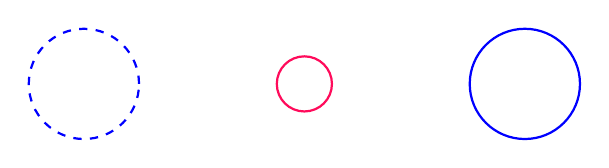
\begin{tikzpicture}[scale=0.7, transform shape]
  \coordinate (AT1) at (0,0);
\coordinate (AT2) at (8,0);
\coordinate (B) at (4,0);

\draw node[fig,
  circle,
  minimum size=2cm,
  draw=blue,
  dashed] (a1) at (AT1) {};

\node[fig,
  circle,
  minimum size=2cm,
  draw=blue] (a2) at (AT2) {};

\node[fig,
  circle,
  minimum size=1cm,
  draw=rose] (b) at (B) {};


\end{tikzpicture}

  \caption{Le phénomène du tunneling}
  \label{tunneling1}
\end{figure}

On pourrait envisager de diminuer la durée du pas de temps
d'intégration afin de diminuer le risque de tunneling, mais même si un
pas de temps faible améliore la qualité des résultats, il ne pourra
pas être indéfiniment réduit. Il est principalement limité par le
temps de calcul d'une mise à jour du système, puisqu'à partir du
moment o\`u $\deriv t$ est inférieur au temps moyen nécessaire à une
machine pour calculer une itération de la simulation, le programme
perdra son statut d'application temps réel.

Une technique usuellement admise est le lancer de rayons
(\textit{raycasting}) entre les points de la position de départ du
solide et les points de sa position d'arrivée. Si l'un des rayons
touche un autre corps, on sait qu'une collision aurait dû être
détectée et on peut revenir en arrière. Cette méthode présente
pourtant une faiblesse de taille, car le résultat de cette recherche
dépend directement de la concentration de rayons. Si on lance peu de
rayons, on risque de ne pas détecter les corps de petite taille et
donc de les traverser tandis qu'une concentration élevée de rayons
pourrait se réveler regrettable en terme de coûts de calcul.

\begin{figure}
  \centering
  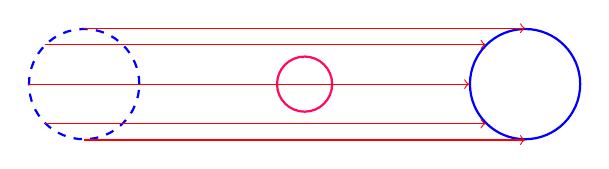
\begin{tikzpicture}[scale=0.7, transform shape]
  \coordinate (AT1) at (0,0);
\coordinate (AT2) at (8,0);
\coordinate (B) at (4,0);

\draw node[fig,
  circle,
  minimum size=2cm,
  draw=blue,
  dashed] (a1) at (AT1) {};

\node[fig,
  circle,
  minimum size=2cm,
  draw=blue] (a2) at (AT2) {};

\node[fig,
  circle,
  minimum size=1cm,
  draw=rose] (b) at (B) {};


  \path[rayon] (a1.north) -- (a2.north);
  \path[rayon] (a1.west) -- (a2.west);
  \path[rayon] (a1.north west) -- (a2.north west);
  \path[rayon] (a1.south) -- (a2.south);
  \path[rayon] (a1.south west) -- (a2.south west);
\end{tikzpicture}

  \caption{Lancer de rayons pour la détection de tunneling}
  \label{tunneling2}
\end{figure}

La technique de la détection de collision continue (\textit{continuous
  collision detection}) permet de contrôler de façon certaine tout
phénomène de tunneling. L'idée est la suivante : soit deux corps $A$
et $B$ dont l'on veut détecter l'éventuelle collision. On construit
deux volumes fantômes $C_A$ et $C_B$ englobant tous les points par
lesquels passent respectivement $A$ et $B$ entre deux
intégrations. Ces volumes n'interviendront pas dans les collisions des
autres objets de la simulation, et on vérifie simplement s'ils entrent
tous deux en collision. Si tel est le cas, alors on sait qu'il est
possible qu'un tunneling se soit produit et on peut revenir en arrière
jusqu'à ce que le problème soit résolu. Pour accélérer cette phase, il
est envisageable d'utiliser des boîtes englobantes de la même façon
que lors de la détection grossière de collision. L'un des avantages
majeurs de cette méthode, en plus de sa certitude de ne manquer aucun
tunneling, est sa simplicité de mise en place puisque toutes les
routines de détection et de retour en arrière utilisées ont déjà été
écrites et entrent en jeu dans le fonctionnement de base du moteur
physique.

\begin{figure}
  \centering
  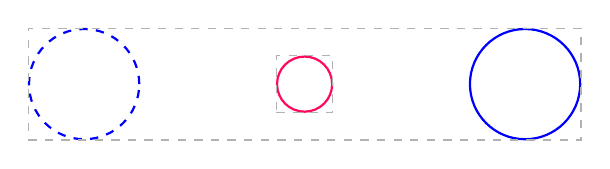
\begin{tikzpicture}[scale=0.7, transform shape]
  \coordinate (AT1) at (0,0);
\coordinate (AT2) at (8,0);
\coordinate (B) at (4,0);

\draw node[fig,
  circle,
  minimum size=2cm,
  draw=blue,
  dashed] (a1) at (AT1) {};

\node[fig,
  circle,
  minimum size=2cm,
  draw=blue] (a2) at (AT2) {};

\node[fig,
  circle,
  minimum size=1cm,
  draw=rose] (b) at (B) {};


  \coordinate (a1n) at ($(a1.north)+(0,0.2)$);
  \coordinate (a2s) at ($(a2.south)+(0,-0.2)$);

  \node[fit=(a1) (a2),
    inner sep=0,
    draw=gris,
    dashed] (aabb1) {};

  \node[fit=(b),
    inner sep=0,
    draw=gris,
    dashed] (aabb2) {};
\end{tikzpicture}

  \caption{Boîtes englobantes pour la détection de tunneling}
  \label{tunneling3}
\end{figure}

\subsubsection{Partitionnement de l'espace}

Comme mis en avant tout au long de ce rapport, on cherche à concevoir
un moteur physique dont la rapidité d'éxécution est un facteur
déterminant. Dans cette optique, il est primordial d'optimiser les
routines géométriques entrant en jeu mais aussi d'éviter leur
exécution inutile dès que possible. La détection des collisions entre
les corps qui peuplent notre système se déroule en deux étapes : une
détection grossière visant à vérifier de façon économique si deux
objets se touchent et une détection fine servant à confirmer ou à
infirmer de façon sûre ce résultat. Bien que la détection grossière
soit peu coûteuse en termes de calcul, elle est éxécutée pour $n$
corps au minimum $\frac{n(n-1)}{2}$ fois à chaque itération, et ce
sans compter les détections de collision exécutées pendant la
recherche dichotomisuqe de l'état de contact. Pourtant, il est très
souvent inutile de détecter si deux objets sont en situation
d'interpénétration, par exemple lorsque la distance les séparant est
grande. Il serait tout à notre avantage d'ajouter au moteur une couche
supplémentaire tenant compte de ces disparités spatiales pour
accélérer la phase de détection de collision.

Le principe général du partitionnement de l'espace (\textit{spatial
  partitioning}) est de subdiviser l'environnement de la simulation en
sous-espaces. La répartition des corps dans ces sous-espaces dépend
bien évidemment de leur position dans le repère global mais aussi du
volume qu'ils occupent. On est certain que seules les entités
appartenant à un même sous-espace peuvent interagir entres elles, on
dispose donc d'une aide quant au choix des objets entre lesquels
vérifier si collision il y a.

Sous sa forme la plus simple, le partitionnement de l'espace prend la
forme d'une grille de taille fixe dans les cases de laquelle les corps
de la simulation sont répartis. L'aspect statique d'une telle
structure présente plusieurs inconvénients majeurs, notamment le fait
que le gain de performance variera fortement selon le nombre d'objets
considérés, leur taille et la finesse de la grille. Par exemple, si
une grille a des cases trop grandes, chacune contiendra de nombreux
objets et le gain de performance sera peu flagrant. Si au contraire
les cases de la grille sont trop petites, les plus grands objets ne
pourront pas rentrer dans leur intégralité à l'intérieur d'une unique
case. Une solution à ce problème est de ranger un même objet dans
plusieurs cases adjacentes de la grille, mais une fois encore, si des
corps sont démultipliés de la sorte, le temps de maintenance d'une
telle structure sera augmenté.

Une variante plus subtile de partitionnement de l'espace est
l'utilisation d'\textit{octrees} (\textit{quadtrees} en deux
dimensions) \cite{millington}. Cette structure de données prend la forme d'un arbre
représentant l'espace à subdiviser. Chaque n\oe ud de l'arbre possède
huit fils, chacun correspondant à un octant du volume de leur père. La
racine de l'arbre est associée au volume complet de l'environnement
que l'on souhaite diviser. Lorsqu'un corps est introduit dans la
simulation, il faut le ranger dans l'arbre. Pour ce faire, on part de
la racine et on descend récursivement jusqu'à une feuille de l'arbre
en se guidant dans les embranchements selon la position et le volume
de l'objet à insérer. L'octree n'est pas nécessairement équilibré et
plus une zone contient de corps et plus elle pourra être subdivisée.

Cette structure sert à stocker les corps de la simulation, et si nous
l'implémentions elle remplacerait la liste qui contient nos objets et
dont l'ordre est actuellement arbitraire. Elle devient
particulièrement intéressante lors de la phase de détection de
collision car il n'est plus désormais nécessaire de tester tous les
corps deux à deux; il suffit de vérifier les collisions entre les
corps du même sous-espace, autrement dit avec tous ceux contenus dans
la même feuille.


\bibliographystyle{apalike}
\bibliography{references}

\end{document}
